	\section{Análise da Legislação}
	Este capítulo tem como objetivo analisar de forma sucinta os instrumentos legais (leis, normas e regulamentos) que direta e/ou diretamente se relacionam com a gestão dos resíduos sólidos nas esferas federal, estadual e municipal, e que serão posteriormente submetidos a uma análise integrada, de forma que sejam identificadas compatibilidades. Esta análise se faz necessária para embasar a elaboração do Plano Municipal de Gestão Integrada de Resíduos Sólidos (PMGIRS) de Monteiro Lobato, verificando sua conformidade com as premissas legais aplicáveis, possibilitando a este importante instrumento de gestão condições para apontar quais adequações gerais e/ou complementações devem ser promovidas no arcabouço legal do município na temática relacionada à limpeza urbana e ao manejo de resíduos sólidos.
	
	\subsection{Legislação Federal}
	A Constituição Federal de 1988 é a lei fundamental e suprema do Brasil, servindo de parâmetro a toda a legislação brasileira \cite{do1988constituiccao}. Em seu artigo 225, a constituição impõe ao poder público e à coletividade o dever de defender e preservar o meio ambiente mantendo-o como de direito de todos, ecologicamente equilibrado. A partir da promulgação da CF, uma série de instrumentos legais na alçada do saneamento básico foram elaborados, com o objetivo de melhoria da qualidade ambiental e de prestação dos serviços, garantindo o acesso universal ao sistema, com controle social.
	
	A Política Nacional de Meio Ambiente (PNMA), instituída pela Lei Federal nº 6938 de 1981, fornece objetivos, instrumentos e diretrizes da PNRS e cria o Sistema Nacional do Meio Ambiente (SISNAMA) e o Conselho Nacional de Meio Ambiente (CONAMA) \cite{machado2012principios}. Dentre as regulações contidas na Lei n.º 6.938/81, em seu Art. 2º estão descritos os princípios orientadores na busca do cumprimento de seus objetivos. Um destes princípios é a ação governamental que objetiva a manutenção do equilíbrio ecológico, considerando então que o meio ambiente é um patrimônio público de uso coletivo e deve ser necessariamente protegido. Uma das formas de promover a preservação, a recuperação e a revitalização do meio ambiente são por meio da gestão adequada dos resíduos sólidos. O instrumento adequado para o planejamento estratégico municipal da gestão de resíduos é o PMGIRS e este deve constituir uma preocupação do Poder Público alinhando assim aos princípios da PNMA.
	
	A Política Nacional de Educação Ambiental (PNEA) estabelece, em seu artigo 1º, que a educação ambiental deve ter a finalidade de construir valores sociais, conhecimentos, habilidades, atitudes e competências voltadas para a conservação do meio ambiente. Fica previsto por meio do Art. 3º e Art. 5º o direito a todos à educação ambiental e delegando as ações e disseminação de informação as instituições educativas, órgãos integrantes do Sistema Nacional de Meio Ambiente, meios de comunicação de massa e à sociedade, conforme os incisos II, III, IV e VI respectivamente. Desta forma, a lei \cite{L979597:online} prevê uma mobilização entre educadores ambientais, entidades e sociedade civil. São os objetivos dessa mobilização: o desenvolvimento de uma compreensão integrada do meio ambiente, o fortalecimento da consciência crítica sobre a problemática ambiental e social, além da garantia de democratização das informações ambientais.  Nesse sentido, os dizeres desta lei são de grande valia para a definição de estratégias de mobilização previstas durante a construção de um PMGIRS dessa forma é possível consolidar a gestão integrada dos resíduos sólidos do município de maneira responsável, e com o acesso à informação a todos envolvidos.
	
	A Política Nacional de Saneamento Básico estabelece as diretrizes nacionais para o saneamento básico. Um de seus objetivos é priorizar planos, programas e projetos que visem à implantação e ampliação dos serviços e ações de saneamento básico nas áreas ocupadas por populações de baixa renda. Em seu artigo 2, a referida política estabelece que abastecimento de água, esgotamento sanitário, limpeza urbana e manejo dos resíduos sólidos devem ser realizados de formas adequadas para garantir a saúde pública e a proteção do meio ambiente. O seu artigo 3 define o saneamento básico:
	
	A Política Nacional de Saneamento Básico condiciona a existência de um Plano Nacional de Saneamento Básico (PNSB). De acordo com a referida lei, o PNSB deve abranger as soluções para o abastecimento de água, o esgotamento sanitário, o manejo de resíduos sólidos e o manejo de águas pluviais, além de outras ações de saneamento básico. O Art. 8-C da Lei Nº 11.445 define como titulares dos serviços públicos de saneamento básico os Municípios e o Distrito Federal. Os titulares poderão delegar a organização, a regulação, a fiscalização e a prestação desses serviços. Torna-se fundamental uma mobilização dos Municípios em prol da construção do Plano Municipal de Saneamento Básico, que será um instrumento indispensável de política pública no que tange o saneamento básico.
	
	A PNRS considera o PMGIRS, cujo conteúdo mínimo está descrito em seu Art. 19, como um dos instrumentos mais importantes para a gestão de resíduos sólidos municipais. Além disso, a elaboração do PMGIRS é condição para que os municípios tenham acesso a recursos da União para empreendimentos e serviços de manejo de resíduos sólidos e limpeza urbana.
	 
	O Decreto 7404/2010 estabelece normas para execução e regulamentação da PNRS. Este documento abrange um acervo de ferramentas eficazes na gestão de resíduos sólidos como: metas graduais, estudos periódicos, modelo de responsabilidade compartilhada, linha de financiamento para a reciclagem e melhorias das condições de trabalho dos catadores. Além disso o decreto visa a construção de um Conselho Interministerial com o objetivo de dar suporte a estruturação e implementação da PNRS, podendo então estabelecer outras regulamentações especificas de acordo com as necessidades. Nos Art. 46 e Art. 48 deste decreto fica estabelecido como obrigação dos Estados e Municípios a elaboração e execução de Plano de Gestão Integrada.
	
	A PNRS relaciona-se com a Política Nacional sobre Mudança do Clima (Lei nº 12.187/2009) que tem como uma de suas metas alcançar o índice de reciclagem de resíduos de 20\% em 2015. Até o momento da elaboração do plano não foram encontradas informações sobre o cumprimento ou não das metas estabelecidas.  
	
	A Lei Federal de Consórcios Públicos, dispõe, em seu artigo 1, sobre normas gerais para a União, os Estados, o Distrito Federal e os Municípios contratarem consórcios públicos para a realização de objetivos de interesse comum. Esta lei é de grande importância para a construção do PMGIRS já que os municípios ou microrregiões que optam por consórcios possuem prioridade ao acesso de recursos da União.
	
	O conjunto das leis federais analisadas na íntegra, bem como as resoluções, normas técnicas, instruções normativas, programas, políticas, planos, portarias, decretos e a Constituição Federal de 1988 encontram-se listadas e resumidas no Apêndice A deste documento. 
	No \autoref{quadro:deliconama} encontra-se o descritivo das principais deliberações do CONAMA no âmbito federal que direta e/ou indiretamente se relacionam com a gestão de resíduos sólidos.
	
	\renewcommand\LTcaptype{quadro}
	\begin{center}
		\begin{longtable}{|p{0.3\textwidth}|p{0.7\textwidth}|}
			\caption{\label{quadro:deliconama}Principais deliberações do CONAMA no âmbito federal que direta e/ou indiretamente se relacionam com a gestão de resíduos sólidos.}\\
			\hline
			\textbf{NORMATIVO} & \textbf{DESCRIÇÃO} \\
			\hline
			\endfirsthead
			\multicolumn{2}{c}%
			{\quadroname\space\ref{quadro:arclsp}\ -- \textit{Continuação da pagina anterior}} \\
			\hline
			\textbf{LEI} & \textbf{DESCRITIVO}\\
			\hline
			\endhead
			
			\hline \multicolumn{2}{r}{\textit{Continua na próxima página}} \\
			\endfoot
			\hline
			\endlastfoot
			Resolução CONAMA n.  5, 05 de agosto de 1993 & Dispõe sobre o gerenciamento de resíduos sólidos gerados nos portos, aeroportos, terminais ferroviários e rodoviários. \\
			\hline
			Resolução   CONAMA   n.   275, de 25 de abril de 2001 & Estabelece  o  código  de  cores  para  os  diferentes  tipos  de  resíduos,  a  ser adotado  na  identificação  de  coletores  e  transportadores,  bem  como  nas campanhas informativas para a coleta seletiva. \\
			\hline
			Resolução   CONAMA   n.   307, de 5 de julho de 2002 & Estabelece diretrizes, critérios e procedimentos para a gestão dos resíduos da construção civil. \\
			\hline
			Resolução   CONAMA   n.   313, de 29 de outubro de 2002 & Dispõe sobre o Inventário Nacional de Resíduos Sólidos Industriais. \\
			\hline
			Resolução   CONAMA   n.   334, de 3 de abril de 2003 & Dispõe     sobre     os     procedimentos     de     licenciamento     ambiental     de estabelecimentos   destinados   ao   recebimento   de   embalagens   vazias   de agrotóxicos. \\
			\hline
			Resolução   CONAMA   n.   348, de 16 de agosto de 2004 & Altera  a  Resolução  CONAMA  n.  307,  de  5  de  julho  de  2002,  incluindo  o amianto na classe de resíduos perigosos. \\
			\hline
			Resolução   CONAMA   n.   358, de 29 de abril de 2005 & Dispõe sobre o tratamento e a disposição final dos resíduos dos serviços de saúde e dá outras providências. \\
			\hline
			Resolução   CONAMA   n.   362, de 23 de junho de 2005 & Dispõe  sobre  o  recolhimento,  coleta  e  destinação  final  de  óleo  lubrificante usado ou contaminado. \\
			\hline
			Resolução   CONAMA   n.   401, de 4 de novembro de 2008 & Estabelece os limites máximos de chumbo, cádmio e mercúrio para pilhas e baterias comercializadas no território nacional e os critérios e padrões para o seu gerenciamento ambientalmente adequado, e dá outras providências. \\
			\hline
			Resolução   CONAMA   n.   404, de 11 de novembro de 2008 & Estabelece  critérios  e  diretrizes  para  o  licenciamento  ambiental  de  aterro sanitário de pequeno porte de resíduos sólidos urbanos. \\
			\hline
			Resolução   CONAMA   n.   411, de 6 de maio de 2009 & Dispõe  sobre  procedimentos  para  inspeção  de  indústrias  consumidoras  ou transformadoras  de produtos e subprodutos  florestais  madeireiros  de origem nativa, bem como os respectivos padrões de nomenclatura e coeficientes de rendimento volumétricos, inclusive carvão vegetal e resíduos de serraria. \\
			\hline
			Resolução   CONAMA   n.   416, de 30 de setembro de 2009 & Dispõe  sobre  a  prevenção  à  degradação  ambiental  causada  por  pneus inservíveis   e   sua   destinação   ambientalmente   adequada,   e   dá   outras providências. \\
			\hline
			Resolução   CONAMA   n.   465, de 5 de dezembro de 2014 & Dispõe  sobre  os  requisitos  e  critérios  técnicos  mínimos  necessários  para  o licenciamento  ambiental  de  estabelecimentos  destinados  ao  recebimento  de embalagens de agrotóxicos e afins, vazias ou contendo resíduos. \\
			\hline
			Resolução   CONAMA   n.   469, de 29 de julho de 2015 & Altera a Resolução CONAMA n. 307, de 05 de julho de 2002, que estabelece diretrizes, critérios e procedimentos para a gestão dos resíduos da construção civil. \\
			\hline
			Resolução   CONAMA   n.   481, de 3 de outubro de 2017 & Estabelece  critérios  e  procedimentos  para  garantir  o  controle  e  a  qualidade ambiental do processo de compostagem  de resíduos  orgânicos, e dá outras providências. \\
			\hline
			
		\end{longtable}
	\end{center}
	\renewcommand\LTcaptype{table}

	\subsection{Legislação Estadual}
	
	Uma análise da legislação estadual de São Paulo mostrou que são relevantes para a elaboração do PMGIRS de Monteiro Lobato as Políticas Estaduais de Meio Ambiente, Saneamento Básico, Resíduos Sólidos, Educação Ambiental, além da Constituição Estadual. 
	
	A Constituição Estadual, carta magna do Estado de São Paulo, define competências em âmbito estadual, citando, em seu artigo 184, que cabe ao Estado, com a cooperação dos Municípios, orientar a utilização racional de recursos naturais de forma sustentada, compatível com a preservação do meio ambiente. Além disso, o Capítulo IV – do Meio Ambiente, dos Recursos Naturais e do Saneamento, define, em seu artigo 191, que o Estado e os Municípios providenciarão, com a participação da coletividade, a preservação, conservação, defesa, recuperação e melhoria do meio ambiente, em harmonia com o desenvolvimento social e econômico. Ainda, o artigo 193 define a criação de um sistema de administração da qualidade ambiental para o Estado, cujas funções incluem informar a população sobre os níveis de poluição e a qualidade do meio ambiente, promover a educação ambiental e a conscientização pública para a preservação, conservação e recuperação do meio ambiente, além de fiscalizar empreendimentos que, direta ou indiretamente, possam causar degradação do meio ambiente.
	
	Ainda no Capítulo IV, a seção IV – do Saneamento, define a criação e desenvolvimento de mecanismos institucionais e financeiros, destinados a assegurar os benefícios do saneamento à totalidade da população; a prestação de assistência técnica e financeira aos Municípios, para o desenvolvimento dos seus serviços; a orientação técnica para os programas visando ao tratamento de resíduos sólidos, e fomento à implantação de soluções comuns, mediante planos regionais de ação integrada.
	
	Seguindo esta mesma linha, está a Lei Estadual nº 7.750/1992, que dispõe sobre a Política Estadual de Saneamento Básico e dá outras providências, visando fornecer subsídios para o planejamento e a execução das ações, obras e serviços de Saneamento no Estado, respeitada a autonomia dos Municípios. Seu objetivo é aumentar a salubridade ambiental, por meio do abastecimento de água potável, coleta e disposição sanitária de resíduos líquidos, sólidos e gasosos, promoção da disciplina sanitária do uso e ocupação do solo, drenagem urbana, controle de vetores de doenças e demais serviços e obras especializados.
	
	A mesma lei determina que os municípios devem realizar o gerenciamento das instalações e serviços de saneamento essencialmente municipais, tais como os serviços e obras de expansão urbana horizontal e vertical, pavimentação, disposição de resíduos, drenagem de águas pluviais, uso e ocupação do solo e demais atividades de natureza tipicamente local.
	
	Quanto à gestão dos resíduos sólidos, a principal lei que rege esta matéria em âmbito estadual é a Lei Estadual nº 12.300/2006,  que Institui a Política Estadual de Resíduos Sólidos (PERS), regulamentada pelo Decreto Estadual nº 54.645, de 5 de agosto de 2009. Essa lei define princípios, diretrizes, objetivos e instrumentos para a gestão integrada e compartilhada de resíduos sólidos, com vistas à prevenção e ao controle da poluição, à proteção e à recuperação da qualidade do meio ambiente, e à promoção da saúde pública, de modo que seja assegurado o uso adequado dos recursos ambientais no Estado de São Paulo.
	
	De acordo com o Artigo 13 desta lei, a gestão dos resíduos sólidos urbanos deverá ser feita pelos Municípios e, preferencialmente, de forma integrada e regionalizada contando com a cooperação do Estado e participação dos organismos da sociedade civil, estimulando a busca de soluções consorciadas e a solução conjunta dos problemas de gestão de resíduos de todas as origens e o fomento à implantação do sistema de coleta seletiva nos municípios, tendo em vista a máxima eficiência e a adequada proteção ambiental com vista à saúde pública. A referida lei também estabelece a elaboração dos Planos Regionais de Gerenciamento de Resíduos Sólidos; de Planos dos Geradores; de Inventário Estadual de Resíduos Sólidos e do Sistema Declaratório Anual de Resíduos Sólidos.
	
	O Plano de Resíduos Sólidos do Estado de São Paulo fornece ações de apoio à gestão municipal de resíduos sólidos, às atividades de reciclagem, coleta seletiva, destinação ambientalmente correta dos resíduos sólidos e às ações de educação ambiental, objetivando provocar mudanças positivas nos hábitos e consumo da população do estado.
	
	O Estado de São Paulo também conta com a Comissão Estadual de Gestão de Resíduos Sólidos, instituída pelo Decreto Estadual nº 54.645 de 2009 e que, segundo seu artigo 26, possui as seguintes atribuições:
	
	\trecholei{“Art 26 - (...) I - cooperar na elaboração e participar na execução do plano de resíduos sólidos a que alude o artigo 6º deste decreto;
		II - Propor, em conjunto com instituições de normalização, quando necessário, padrões de qualidade para materiais obtidos por meio da reciclagem, para fins de certificação ambiental de produtos;
		III - estabelecer, em conjunto com os setores produtivos, instrumentos e mecanismos econômicos para fomentar a gestão e o gerenciamento dos resíduos sólidos.”}
	
	Outra legislação estadual que se relaciona com a PERS é a Resolução nº 45/2015 da Secretaria do Meio Ambiente (SMA) que aborda a logística reversa , em seu Artigo 2º:
	
	\trecholei{“Artigo 2º - São obrigados a estruturar e implementar sistemas de logística reversa, mediante retorno dos produtos e embalagens após o uso pelo consumidor, de forma independente do serviço público de limpeza urbana e de manejo dos resíduos sólidos, os fabricantes, importadores, distribuidores e comerciantes dos produtos que, por suas características, exijam ou possam exigir sistemas especiais para acondicionamento, armazenamento, coleta, transporte, tratamento ou destinação final, (...)”}
	
	De forma complementar ao discorrido, uma série de dispositivos legais coexistem no arcabouço legislativo do Estado de São Paulo que tratam de matérias especificas e correlatas a gestão dos resíduos sólidos, conforme exposto no \autoref{quadro:arclsp} a seguir.
	
	\renewcommand\LTcaptype{quadro}
	\begin{center}
		\begin{longtable}{|p{0.3\textwidth}|p{0.7\textwidth}|}
			\caption{\label{quadro:arclsp}Arcabouço legislativo do Estado de São Paulo que se relacionam diretamente ou indiretamente com os resíduos sólidos.}\\
			\hline
			\textbf{LEI} & \textbf{DESCRITIVO}\\
			\hline
			\endfirsthead
			\multicolumn{2}{c}%
			{\quadroname\space\ref{quadro:arclsp}\ -- \textit{Continuação da pagina anterior}} \\
			\hline
			\textbf{LEI} & \textbf{DESCRITIVO}\\
			\hline
			\endhead
			
			\hline \multicolumn{2}{r}{\textit{Continua na próxima página}} \\
			\endfoot
			\hline
			\endlastfoot
			Lei Estadual n. 2.627, de 20 de janeiro de 1954 & Cria e organiza o Departamento de Águas e Esgotos como autarquia, extingue a Repartição de Águas e Esgotos de São Paulo e dá outras providências. \\
			\hline
			Lei Estadual n. 10.107, de 8 de maio de 1968 & Dispõe sobre a criação do Fundo Estadual de Saneamento Básico e dá outras providências. \\
			\hline
			Decreto Estadual n. 50.079, de 24 de julho de 1968 & Dispõe  sobre  a  constituição  do  Centro  Tecnológico  de  Saneamento  Básico, prevista  na  Lei  Estadual  n.  10.107,  de  8  de  maio  de  1968,  e  dá  outrasprovidências. \\
			\hline
			Decreto-Lei  Estadual  n.  145, de 8 de agosto de 1969 & Dispõe  sobre  a  criação  do  Parque  Estadual  de  Jacupiranga  e  dá  outras providências. \\
			\hline
			Lei Estadual n.  118, de 29 de junho de 1973 & Autoriza  a  constituição  de  uma  sociedade  por  ações,  sob  a  denominação  de CETESB  –  Companhia  Estadual  de  Tecnologia  de  Saneamento  Básico  e  de Controle de Poluição das Águas, e dá providências correlatas. \\
			\hline
			Lei Estadual n.  119, de 29 de junho de 1973 & Autoriza  a  constituição  de  uma  sociedade  por  ações,  sob  a  denominação  de Companhia de Saneamento Básico do Estado de São Paulo  – SABESP, e dá providências correlatas. \\
			\hline
			Lei Estadual n. 898, de 18 de dezembro de 1975 & Disciplina o uso de solo para a proteção dos mananciais, cursos e reservatórios de  água  e  demais  recursos  hídricos  de  interesse  da  Região  Metropolitana  da Grande São Paulo e dá providências correlatas. \\
			\hline
			Lei Estadual n.  997, de 31 de maio de 1976 & Dispõe sobre o controle da poluição do meio ambiente. \\
			\hline
			Decreto  Estadual  n.  8.468,  de 8 de setembro de 1976 & Aprova o Regulamento da Lei n. 997, de 31 de maio de 1976, que dispõe sobre a prevenção e o controle da poluição do meio ambiente. \\
			\hline
			Lei  Estadual  1.172,  de  17  de novembro de 1976 & Delimita as áreas de proteção relativas aos mananciais, cursos e reservatórios de água, a que se refere o Artigo 2.º da Lei n. 898, de 18 de dezembro de 1975, estabelece normas de restrição de uso do solo em tais áreas e dá providências correlatas. \\
			\hline
			Decreto  Estadual  n.  9.714,  de 19 de abril de 1977 & Aprova o Regulamento das Leis n.º 898, de 18 de dezembro de 1975 e n.º 1172, de 17 de novembro de 1976, que dispõe sobre o disciplinamento do uso do solo para a proteção aos mananciais da Região Metropolitana da Grande São Paulo. \\
			\hline
			Lei Estadual n. 1.817, de 27 de outubro de 1978 & Estabelece   os   objetivos   e  as   diretrizes   para   o  desenvolvimento  industrial metropolitano e disciplina o zoneamento industrial, a localização, a classificação e  o  licenciamento  de  estabelecimentos  industriais  na  Região  Metropolitana da Grande São Paulo e dá providências correlatas. \\
			\hline
			Lei Estadual n. 2.252, de 20 de dezembro de 1979 & Altera a redação de dispositivos da Lei n. 440, de 24 de setembro de 1974, que dispõe  sobre  o  Imposto  de  Circulação  de  Mercadorias,  e  dá  providências correlatas.\newline{}Artigo  1º  –  Passam  a  vigorar  com  a  seguinte  redação  os  dispositivos  adiante enumerados, todos da Lei n. 440, de 24 de setembro de 1974:\newline{}IV – o Artigo 11:\newline{}Artigo 11 – São sujeitos passivos por substituição:\newline{}V – o contribuinte que realizar as operações abaixo indicadas, relativamente ao imposto devido nas anteriores saídas de papel usado e aparas de papel, sucata de  metais,  cacos  de  vidro,  retalhos,  fragmentos  e  resíduos  de  plástico,  de borracha ou de tecido, promovidas por quaisquer estabelecimentos:\newline{}a) saída de produtos fabricados com essas mercadorias;\newline{}b) saída dessas mercadorias com destino a estabelecimento localizado em outra unidade da Federação. \\
			\hline
			Decreto Estadual n. 20.903, de 26 de abril de 1983 & Cria o Conselho Estadual do Meio Ambiente - CONSEMA. \\
			\hline
			Lei Estadual n. 4.435, de 5 de dezembro de 1984 & Veda  a  instalação  de  depósito  de  lixo,  usinas  de  beneficiamento  de  resíduos sólidos e aterros sanitários em área que especifica. \\
			\hline
			Lei Estadual n. 4.529, de 18 de janeiro de 1985 & Dispõe  sobre  o  uso  e  ocupação  do  solo  na  Região  da  Serra  do  Itapeti  com vistas  à  proteção  e  melhoria  da  qualidade  do  meio  ambiente  na  Região Metropolitana de São Paulo. \\
			\hline
			Lei Estadual n. 4.882, de 3 de dezembro de 1985 & Traz  o  conceito  de  Saneamento  Geral  como  ações  e  obras  integradas  para viabilizar  ou   manter,  na   Região   Metropolitana,  infraestrutura  sanitária   que assegure condições de higiene, saúde e bem-estar as comunidades, mediante o abastecimento  de  águas,  instalação  de  redes  de  esgoto,  coleta  e  disposição final  de  resíduos.  Investimentos  com  recursos  do  FAE  –  Fundo  de  Águas  e Esgoto. \\
			\hline
			Lei Estadual n. 5.597, de 6 de fevereiro de 1987 & Estabelece normas e diretrizes para o zoneamento industrial no Estado de São Paulo e dá providências correlatas. \\
			\hline
			Lei Estadual n. 6.134, de 2 de junho de 1988 & Dispõe sobre a preservação dos depósitos naturais de águas subterrâneas do Estado de São Paulo e dá outras providências.\newline{}Artigo 5.º – Os resíduos líquidos, sólidos ou gasosos, provenientes de atividades agropecuárias,   industriais,   comerciais   ou   de   qualquer   outra   natureza,   só poderão  ser  conduzidos  ou  lançados  de  forma  a  não  poluírem  as  águas\newline{}subterrâneas. \\
			\hline
			Constituição  Estadual  de  São Paulo,   de   5   de   outubro   de 1989 & Artigo  215  –  A  lei  estabelecerá  a  política  das  ações  e  obras  de  saneamento básico no Estado, respeitando os seguintes princípios:\newline{}I  –  criação  e  desenvolvimento  de  mecanismos  institucionais  e  financeiros, destinados a assegurar os benefícios do saneamento à totalidade da população; II  –  prestação  de  assistência  técnica  e  financeira  aos  Municípios,  para  o desenvolvimento dos seus serviços;\newline{}III – orientação técnica para os programas visando ao tratamento  de despejos urbanos  e  industriais  e  de  resíduos  sólidos,  e  fomento  à  implantação  de soluções comuns, mediante planos regionais de ação integrada.\newline{}Artigo  216  –  O  Estado  instituirá,  por  lei,  plano  plurianual  de  saneamento estabelecendo as diretrizes e os programas para as ações nesse campo.\newline{}§ 1º – O plano, objeto deste artigo, deverá respeitar as peculiaridades regionais e locais e as características das bacias hidrográficas e dos respectivos recursos hídricos.\newline{}§  2º  –  O  Estado  assegurará  condições  para  a  correta  operação,  necessária ampliação   e   eficiente   administração   dos   serviços   de   saneamento   básico prestados por concessionária sob seu controle acionário.\newline{}§ 3º – As ações de saneamento deverão prever a utilização racional da água, do solo e do ar, de modo compatível com a preservação e melhoria da qualidade\newline{}da saúde pública e do meio ambiente e com a eficiência dos serviços públicos de saneamento. \\
			\hline
			Lei Estadual n. 7.452, de 26 de julho de 1991 & Estabelece  penalidades  administrativas  em  casos  de  danos  aos  bens  de  uso comum sob administração do órgão rodoviário estadual.\newline{}Artigo  1º  –  Constituem  infração  administrativa,  punível  com  multa  fixada  na forma deste artigo, os seguintes comportamentos, causadores de dano, efetivo ou potencial, aos bens públicos afetos ao serviço rodoviário estadual:\newline{} XV – descarregar, lançar, derrubar, depositar ou abandonar, em qualquer parte da  estrada,  sucata,  lixo,  entulho,  lenha,  cana–de–açúcar, bem  como  qualquer outro material ou carga: Pena: multa de 5 (cinco) a 10 (dez) UFESP. \\
			\hline
			Lei Estadual n. 7.641, de 19 de dezembro de 1991 & Dispõe  sobre  a proteção  ambiental  das  bacias  dos  Rios  Pardo,  Moji  Guaçu  e Médio Grande, estabelece critérios para o uso e ocupação do solo nesta área.\newline{}Das Disposições Finais e Transitórias:\newline{}Artigo 2º – Enquanto não for estabelecido o macrozoneamento a que se refere o inciso   I,   do   artigo   2º,   a   instalação   de   estabelecimentos   industriais   e agroindustriais deverá obedecer, além dos critérios contidos no corpo desta lei, as seguintes normas:\newline{}I   –   será   proibida   a   instalação   de   polos   petroquímicos,   carboquímicos, cloroquímicos e indústrias nucleares;\newline{}II  –  ficam  condicionados  à  apresentação  de  EIA/RIMA  (Estudo  de  Impacto Ambiental e respectivo Relatório de Impacto de Meio Ambiente) à aprovação do Conselho  Estadual  do  Meio  Ambiente,  os  empreendimentos  enquadrados  nas seguintes categorias:\newline{}a)  –  indústrias  que  queimem  mais  de  25  (vinte  e  cinco)  unidades  padrão  de combustível por dia, calculadas na forma do método "A”;\newline{}b) – indústrias que produzam, estoquem e disponham de mais de 400kg/mês de resíduos perigosos, conforme definidos pela NBR 10.004 Resíduos Sólidos, de setembro de 1977, da Associação Brasileira de Normas Técnicas;\newline{}c) – indústrias que tenham alto potencial poluidor da atmosfera, determinado na forma do método "B". \\
			Lei Estadual n. 7.663, de 30 de dezembro de 1991 & Estabelece normas de orientação à Política Estadual de Recursos Hídricos bem como ao Sistema Integrado de Gerenciamento de Recursos Hídricos. \\
			\hline
			Lei Estadual n. 7.750, de 31 de março de 1992 & Dispõe sobre a Política Estadual de Saneamento e dá outras providências. \\
			\hline
			Lei Estadual n. 8.211, de 8 de janeiro de 1993 & Institui Zona Industrial na Região Metropolitana da Grande São Paulo. \\
			\hline
			Lei Estadual n. 8.275, de 29 de março de 1993 & Cria a Secretaria de Estado de Recursos Hídricos, Saneamento e Obras, altera a  denominação  da  Secretaria  de  Energia  e  Saneamento  e  dá  providências correlatas. \\
			\hline
			Decreto Estadual n. 37.300, de 25 de agosto de 1993 & Regulamenta o Fundo Estadual de Recursos Hídricos  - FEHIDRO, criado pela Lei n. 7.663, de 30 de dezembro de 1991. \\
			\hline
			Lei Estadual n. 8.794, de 19 de abril de 1994 & Autoriza  a  Fazenda  do  Estado  a  adotar  medidas  de  privatização  e  eventual extinção da Ceagesp – Companhia de Entrepostos e Armazéns Gerais de São Paulo, e dá providências correlatas.\newline{}Artigo  6º  –  Na  hipótese  de  concessão  de  entreposto  do  sistema  estadual  de abastecimento,  o  edital  de  licitação  e  o  respectivo  instrumento  devem  conter cláusulas ou condições que:\newline{}I – preservem a eficiência do sistema estadual de abastecimento e as atividades próprias da Secretaria de Agricultura e Abastecimento, especialmente quanto ao seguinte:\newline{}e) análise de resíduos. \\
			\hline
			Lei Estadual n. 9.146, de 9 de março de 1995 & Cria  mecanismos  de  compensação  financeira  para  municípios  nos  casos  que especifica e dá outras providências. \\
			\hline
			Lei Estadual n. 9.176, de 2 de outubro de 1995 & Altera a Lei n. 6.374, de 1º de março de 1989, relativamente à sujeição passiva por substituição.\newline{}Artigo 1º, XVI – quanto a papel usado e apara de papel, sucata de metal, casco de vidro, retalho, fragmento e resíduo de plástico, de borracha ou de tecido: o contribuinte  que  realize  as  operações  a  seguir  indicadas,  relativamente  ao imposto     devido     nas     anteriores     saídas     promovidas     por     quaisquer estabelecimentos;\newline{}a) saída de mercadorias fabricadas com esses insumos;\newline{}b) saída dessas mercadorias com destino a outro Estado, ao Distrito Federal ou ao Exterior. \\
			\hline
			Lei Estadual n. 9.193, de 28 de novembro de 1995 & Acrescenta dispositivo à Lei n. 1.817, de 27 de outubro de 1978. \\
			\hline
			Lei Estadual n. 9.338, de 09 de janeiro de 1996 & Institui nas escolas estaduais de 1º e 2º graus a “Semana da Gincana de Coleta de Lixo Reciclável”. \\
			\hline
			Lei Estadual n. 9.472, de 30 de dezembro de 1996 & Disciplina o uso de áreas industriais de que trata o artigo 8º da Lei n. 1.817, de 27/10/1978. \\
			\hline
			Lei Estadual n. 9.477, de 30 de dezembro de 1996 & Altera a Lei n. 997, de 31 de maio de 1976. \\
			\hline
			Lei Estadual n. 9.505, de 11 de março de 1997 & Disciplina as ações e os serviços de saúde dos trabalhadores no Sistema Único de Saúde. \\
			\hline
			Lei Estadual n. 9.509, de 20 de março de 1997 & Dispõe sobre a Política Estadual do Meio Ambiente, seus fins e mecanismos de formulação e aplicação. \\
			\hline
			Lei Estadual n. 9.532, de 24 de abril de 1997 & Institui a "Semana da Coleta Seletiva e Reciclagem do Lixo". \\
			\hline
			Lei Estadual n. 9.866, de 28 de novembro de 1997 & Dispõe  sobre  diretrizes  e  normas  para  a  proteção  e  recuperação  das  bacias hidrográficas dos mananciais de interesse regional do Estado de São Paulo e dá outras providências.\newline{}Seção II da infraestrutura sanitária:\newline{}Artigo  20  –A  implantação  de  sistema  coletiva  de  tratamento  e  disposição  de resíduos sólidos domésticos em APRM será permitida desde que:\newline{}I – seja comprovada a inviabilidade de implantação em áreas situadas fora da APRM;\newline{}II  –  sejam  adotados  sistemas  de  coleta,  tratamento  e  disposição  final,  cujos projetos atendam a normas, índices e parâmetros específicos para as APRMs, a serem estabelecidos pelo órgão ambiental competente; e\newline{}III  –  sejam  adotados,  pelos  Municípios,  programas  integrados  de  gestão  de resíduos sólidos que incluam, entre outros, a minimização dos resíduos, a coleta\newline{}seletiva e a reciclagem. \\
			\hline
			Lei Estadual n. 10.019, de 3 de julho de 1998 & Dispõe sobre o Plano Estadual de Gerenciamento Costeiro. \\
			\hline
			Lei  Estadual  n.  10.083,  de  23 de setembro de 1998 & Dispõe sobre o Código Sanitário do Estado. \\
			\hline
			Lei  Estadual  n.  10.217,  de  19 de janeiro de 1999 & Autoriza   o   Poder   Executivo   a   criar   o   sistema   de   saneamento   básico   e despoluição do rio Tietê. \\
			\hline
			Lei Estadual n. 10.306, de 5 de maio de 1999 & Dispõe sobre a instalação de lixeiras seletivas nas escolas públicas estaduais. \\
			\hline
			Decreto Estadual n. 44.038, de 15 de junho de 1999 & Aprova  Regulamento  fixando  os  procedimentos  relativos  ao  cadastramento  e fiscalização do uso, da aplicação, da distribuição e comercialização de produtos agrotóxicos, seus componentes e afins, no território do Estado de São Paulo e dá providências correlatas. \\
			\hline
			Lei  Estadual  n.  10.478,  de  22 de dezembro de 1999 & Dispõe  sobre  a  adoção  de  medidas  de  defesa  sanitária  vegetal  no  âmbito  do Estado. \\
			\hline
			Lei  Estadual  n.  10.503,  de  17 de fevereiro de 2000 & Dispõe sobre poluição nas rodovias estaduais e dá outras providências. \\
			\hline
			Lei  Estadual  n.  10.522,  de  29 de março de 2000 & Autoriza  o  Poder  Executivo  a  instituir  o  Programa  de  Desenvolvimento  de Atividades   de   Pesquisa   Discente   sobre   Temas   Incorporados   ao   Projeto Pedagógico das Unidades Escolares de Ensino Médio. \\
			\hline
			Lei Estadual n. 10.547, de 2 de maio de 2000 & Define procedimentos, proibições, estabelece regras de execução e medidas de precaução  a  serem  obedecidas  quando  do  emprego  do  fogo  em  práticas agrícolas, pastoris e florestais. \\
			\hline
			Lei  Estadual  n.  10.763,  de  23 de janeiro de 2001 & Dispõe   sobre   medidas   a   serem   adotadas   na   prevenção   e   controle   às inundações. \\
			\hline
			Decreto Estadual n. 45.643, de 26 de janeiro de 2001 & Dispõe   sobre   a   obrigatoriedade   da   aquisição   pela   Administração   Pública Estadual de lâmpadas de maior eficiência energética e menor teor de mercúrio, por tipo e potência, e dá providências correlatas. \\
			\hline
			Lei Estadual n. 10.773, de 1 de março de 2001 & Declara Área de Proteção Ambiental a Bacia Hidrográfica do Rio Batalha. \\
			\hline
			Lei  Estadual  n.  10.855,  de  31 de agosto de 2001 & Dispõe sobre a instituição do "Circuito Turístico da Represa do Jurumirim" e dá providências correlatas.\newline{}Artigo 2º – A implantação do Circuito deve observar os preceitos de adequação da atividade ambientalmente sustentável, como:\newline{}II – prevenção à degradação do ecossistema; III – preservação da biodiversidade;\newline{}IV – tratamento e destinação ambientalmente seguros de resíduos antrópicos;\newline{}V – recuperação das áreas degradadas em virtude da continuidade da visitação e da falta de estratégia anterior. \\
			\hline
			Lei  Estadual  n.  10.856,  de  31 de agosto de 2001 & Cria o Programa de Coleta Seletiva de Lixo nas escolas públicas do Estado de São Paulo e dá outras providências. \\
			\hline
			Lei  Estadual  n.  10.888,  de  20 de setembro de 2001 & Dispõe sobre o descarte final de produtos potencialmente perigosos do resíduo urbano que contenham metais pesados e dá outras providências. \\
			\hline
			Lei  Estadual  n.  11.160,  de  18 de junho de 2002 & Dispõe sobre a criação do Fundo Estadual de Prevenção e Controle da Poluição\newline{}– FECOP \\
			\hline
			Decreto Estadual n. 46.842, de 19 de junho de 2002 & Regulamenta  a  Lei  n.º  11.160,  de  18  de  junho  de  2002,  que  dispõe  sobre  a criação do Fundo Estadual de Prevenção e Controle da Poluição (FECOP). \\
			\hline
			Lei  Estadual  n.  11.165,  de  27 de junho de 2002 & Institui o Código de Pesca e Aquicultura do Estado.\newline{}Seção  II  trata  das  vedações  e  proteção  ao  meio  ambiente,  Artigo  16.  –  Os efluentes  das  redes  de  esgotos  e  os  resíduos  líquidos  ou  sólidos  somente poderão  ser  lançados  às  águas  quando  não  as  tornarem  poluídas,  mediante comprovação através de laudo emitido pelo órgão competente. \\
			\hline
			Lei  Estadual  n.  11.220,  de  24 de julho de 2002 & Dispõe sobre a instituição do Polo Turístico das Cidades Religiosas e dá outras providências.\newline{}Artigo  3º  –  A  implantação  do  Polo  Turístico  das  Cidades  Religiosas  deve observar os preceitos de adequação da atividade ambientalmente sustentável, como:\newline{}I – capacitação dos recursos humanos;\newline{}II – prevenção da degradação do ecossistema; III – preservação da biodiversidade;\newline{}IV – tratamento e destinação ambientalmente seguros de resíduos antrópicos;\newline{}V – recuperação das áreas degradadas, em virtude da continuidade da visitação e da falta de estratégia anterior. \\
			\hline
			Decreto Estadual n. 47.397, de 4 de dezembro de 2002 & Dá nova redação ao Título V e ao Anexo 5 e acrescenta os Anexos 9 e 10, ao Regulamento da Lei n.º 997, de 31 de maio de 1976, aprovado pelo Decreto n.º 8.468, de 8 de setembro de 1976, que dispõe sobre a prevenção e o controle da poluição do meio ambiente. \\
			\hline
			Decreto Estadual n. 47.400, de 4 de dezembro de 2002 & Regulamenta  dispositivos  da Lei  Estadual n.  9.509, de  20 de  março de  1997, referentes ao licenciamento ambiental, estabelece prazos de validade para cada modalidade   de   licenciamento   ambiental   e  condições   para   sua   renovação, estabelece  prazo  de  análise  dos  requerimentos  e  licenciamento  ambiental, institui procedimento obrigatório de notificação de suspensão ou encerramento\newline{}de atividade, e o recolhimento de valor referente ao preço de análise. \\
			\hline
			Lei  Estadual  n.  11.364,  de  28 de março de 2003 & Altera   a   denominação   da   Secretaria   de   Estado   de   Recursos   Hídricos, Saneamento e Obras, e autoriza o Poder Executivo a extinguir a Secretaria de Estado de Energia e dá providências correlatas. \\
			\hline
			Decreto Estadual n. 48.896, de 26 de agosto de 2004 & Regulamenta o Fundo Estadual de Recursos Hídricos  - FEHIDRO, criado pela Lei n. 7.663, de 30 de dezembro de 1991, alterada pela Lei n. 10.843, de 5 de julho de 2001. \\
			\hline
			Lei  Estadual  n.  11.815,  de  23 de dezembro de 2004 & Dispõe sobre a criação de área de Zona de Uso Predominantemente Industrial (ZUPI) no Município de Itapevi. \\
			\hline
			Lei Estadual n. 11.817, de 3 de janeiro de 2005 & Inclui zona de uso predominantemente industrial (ZUPI) no Município de Mauá. \\
			\hline
			Lei  Estadual  n.  12.047,  de  21 de setembro de 2005 & Institui Programa Estadual de Tratamento e Reciclagem de Óleos e Gorduras de Origem Vegetal ou Animal e Uso Culinário. \\
			\hline
			Decreto Estadual n. 50.170, de 4 de novembro de 2005 & Institui o Selo Socioambiental no âmbito da Administração Pública Estadual. \\
			\hline
			Lei  Estadual  n.  12.288,  de  22 de fevereiro de 2006 & Dispõe  sobre  a  eliminação  controlada  dos  PCBs  e  dos  seus  resíduos, descontaminação   de   transformadores,   capacitores   e   demais   equipamentos elétricos que contenham PCBs, e dá providências correlatas. \\
			\hline
			Lei  Estadual  n.  12.300,  de  16 de março de 2006 & Institui a Política Estadual de Resíduos Sólidos e define princípios e diretrizes. \\
			\hline
			Decreto Estadual n. 50.753, de 28 de abril de 2006 & Altera a redação e inclui dispositivos no Regulamento aprovado pelo Decreto n.\newline{}8.468, de 1976, disciplinando a execução da Lei n. 997, de 1976, que dispõe sobre controle da poluição do meio ambiente. \\
			\hline
			Lei Estadual n. 12.528, de 2 de janeiro de 2007 & Obriga  a  implantação  do  processo  de  coleta  seletiva  de  lixo  em  shopping centers e outros estabelecimentos que especifica, do Estado de São Paulo. \\
			\hline
			Lei  Estadual  n.  12.684,  de  26 de julho de 2007 & Proíbe o uso, no Estado de São Paulo de produtos, materiais ou artefatos que\newline{}contenham  quaisquer  tipos  de  amianto  ou  asbesto  ou  outros  minerais  que, acidentalmente, tenham fibras de amianto na sua composição. \\
			\hline
			Lei  Estadual  n.  12.780,  de  30 de novembro de 2007 & Institui a Política Estadual de Educação Ambiental. \\
			\hline
			Decreto Estadual n. 52.455, de 7 de dezembro de 2007 & Aprova  o  regulamento  da  Agência  Reguladora  de  Saneamento  e  Energia  do Estado de São Paulo – ARSESP. \\
			\hline
			Lei Complementar Estadual n. 1.025,  de  7  de  dezembro  de 2007 & Transforma a Comissão de Serviços Públicos de Energia  – CSPE em Agência Reguladora  de  Saneamento  e  Energia  do  Estado  de  São  Paulo  –  ARSESP, dispõe sobre os serviços públicos de saneamento básico e de gás canalizado no Estado, e dá outras providências. \\
			\hline
			Decreto Estadual n. 52.469, de 12 de dezembro de 2007 & Altera  a  redação  de  dispositivos  do  Regulamento  aprovado  pelo  Decreto  n. 8.468, de 8 de setembro de 1976, que dispõe sobre o controle da poluição do meio ambiente, confere nova redação ao artigo 6º do Decreto n. 50.753, de 28 de abril de 2006, e dá providências correlatas. \\
			\hline
			Lei  Estadual  n.  12.802,  de  18 de janeiro de 2008 & Institui o "Dia do Agente do Meio Ambiente". \\
			\hline
			Lei  Estadual  n.  12.810,  de  21 de fevereiro de 2008 & Altera os limites do Parque Estadual de Jacupiranga, criado pelo Decreto-lei n. 145,  de  8  de  agosto  de  1969,  e  atribui  novas  denominações  por  subdivisão, reclassifica, exclui e inclui áreas que especifica, institui o Mosaico de Unidades de Conservação do Jacupiranga e dá outras providências. \\
			\hline
			Decreto Estadual n. 52.895, de 11 de abril de 2008 & Autoriza a Secretaria de Saneamento e Energia a representar o Estado de São Paulo  na  celebração  de  convênios  com  Municípios  paulistas,  ou  consórcio  de Municípios,  visando  à  elaboração  de  planos  de  saneamento  básico  e  sua consolidação no Plano Estadual de Saneamento Básico. \\
			\hline
			Lei Estadual n. 13.123, de 8 de julho de 2008 & Institui o Plano Plurianual para o período de 2008/2011. No capítulo 4.4, sobre Meio Ambiente, trata da atuação o governo paulista para diminuir a geração de resíduos (de lixo a gases de efeito-estufa). \\
			\hline
			Decreto Estadual n. 53.336, de 20 de agosto de 2008 & Aprova  a  Norma  Técnica  sobre  Gerenciamento  de  Resíduos  Perigosos  de Medicamentos em Serviços de Saúde. \\
			\hline
			Lei  Estadual  n.  13.507,  de  23 de abril de 2009 & Dispõe  sobre  o  Conselho  Estadual  de  Meio  Ambiente  –  CONSEMA,  e  dá providências correlatas. \\
			\hline
			Lei Estadual n. 13.542, de 8 de maio de 2009 & Altera a denominação da CETESB – Companhia de Tecnologia de Saneamento Ambiental e dá nova redação aos artigos 2º e 10 da Lei n. 118, de 29 de junho de 1973. \\
			\hline
			Lei  Estadual  n.  13.550,  de  2 junho de 2009 & Dispõe sobre a utilização e proteção da vegetação nativa do Bioma Cerrado no Estado, e dá providências correlatas.\newline{}Artigo  8º  –  Nas  áreas  urbanas,  a  supressão  da  vegetação  do  Bioma  Cerrado para  parcelamento  do  solo  ou  qualquer  edificação,  observado  o  disposto  no Plano  Diretor  do  Município  e  demais  normas  aplicáveis,  dependerá  de  prévia autorização  do  órgão  ambiental  competente  e  deverá  atender  os  seguintes requisitos:\newline{}I  –  preservação  da  vegetação  nativa  em  área  correspondente  a,  no  mínimo, 20\% (vinte por cento) da área da propriedade;\newline{}II – preservação de, no mínimo, 30\% (trinta por cento) da área do fragmento de vegetação  nativa  existente  na  propriedade,  no  caso  de  estágio  inicial  de regeneração, e de, no mínimo, 50\% (cinquenta por cento) da área do fragmento de  vegetação  nativa  existente  na  propriedade,  no  caso  de  estágio  médio  de regeneração, respeitado o disposto no inciso I deste artigo;\newline{}III – averbação à margem da matrícula do imóvel correspondente da vegetação remanescente como área verde, sendo essa providência dispensada  quando a área for inferior a 1.000 $m^2$ (mil metros quadrados). \\
			\hline
			Lei Estadual n. 13.576, de 6 de julho de 2009 & Inclui normas e procedimentos para a reciclagem, gerenciamento e destinação final de lixo tecnológico. \\
			\hline
			Lei Estadual n. 13.577, de 8 de julho de 2009 & Dispõe sobre diretrizes e procedimentos para a proteção da qualidade do solo e gerenciamento de áreas contaminadas, e dá outras providências correlatas. \\
			\hline
			Decreto Estadual n. 54.645, de 5 de agosto de 2009 & Regulamenta dispositivos da Lei nº 12.300 de 16 de março de 2006, que institui a  Política  Estadual  de  Resíduos  Sólidos,  e  altera  o  inciso  I  do  artigo  74  do Regulamento da Lei nº 997, de 31 de maio de 1976, aprovado pelo Decreto nº 8.468, de 8 de setembro de 1976. \\
			\hline
			Lei Estadual n. 13.798, de 9 de novembro de 2009 & Institui a Política de Mudanças Climáticas – PEMC. \\
			\hline
			Decreto Estadual n. 55.565, de 15 de março de 2010 & Dispõe sobre a prestação de serviços públicos de saneamento básico relativos à limpeza  urbana  e  ao  manejo  de  resíduos  sólidos  urbanos  no  Estado  de  São Paulo e dá providências correlatas. \\
			\hline
			Decreto Estadual n. 55.947, de 24 de junho de 2010 & Regulamenta a Lei n. 13.798, de 9 de novembro de 2009, que dispõe sobre a Política Estadual de Mudanças Climáticas (PEMC). \\
			\hline
			Lei  Estadual  n.  14.186,  de  15 de julho de 2010 & Dispõe sobre a coleta, o recolhimento e o destino final das embalagens plásticas de óleos lubrificantes, e dá outras providências correlatas. \\
			\hline
			Lei Complementar Estadual n. 1.139, de 16 de junho de 2011 & Reorganiza  a  Região  Metropolitana  da  Grande  São  Paulo,  cria  o  respectivo Conselho de Desenvolvimento e dá providências correlatas. \\
			\hline
			Lei Estadual n. 14.470, de 22 e junho de 2011 & Dispõe sobre a separação dos resíduos recicláveis descartados pelos órgãos e entidades da administração pública estadual, na forma que especifica. \\
			\hline
			Lei  Estadual  n.  14.487,  de  13 de julho de 2011 & Dispõe sobre organização de cursos de atualização e requalificação profissional de trabalhadores nas atividades que especifica. \\
			\hline
			Decreto Estadual n. 57.479, de 1 de novembro de 2011 & Institui  o  Programa  Estadual  Água  é  Vida  para  localidades  de  pequeno  porte predominantemente   ocupadas   por   população   de   baixa   renda,   mediante utilização  de  recursos  financeiros  estaduais  não  reembolsáveis,  destinados  a obras  e  serviços  de  infraestrutura, instalações  operacionais  e  equipamentos  e dá providências correlatas. \\
			\hline
			Lei Estadual n. 14.687, de 2 de janeiro de 2012 & Institui  o  Programa  pró  conexão  de  subsídio  financeiro  à  população  de  baixa renda   para   a   realização   de   obras   necessárias   à   efetivação   de   ligações domiciliares de esgoto que demandem execução de ramais intradomiciliares. \\
			\hline
			Decreto Estadual n. 57.817, de 28 fevereiro de 2012 & Institui, sob coordenação da Secretaria do Meio Ambiente, o Programa Estadual de   Implementação   de   Projetos   de   Resíduos   Sólidos   e   dá   providências correlatas. \\
			\hline
			Decreto Estadual n. 57.933, de 2 de abril de 2012 & Reorganiza a Secretaria do Meio Ambiente e dá providências correlatas. Artigo 2º - Constituem o campo funcional da Secretaria do Meio Ambiente:\newline{}I - de modo a atuar, no âmbito do Estado de São Paulo, como órgão seccional do Sistema Nacional do Meio Ambiente - SISNAMA, de que trata a Lei federal n. 6.938, de 31 de agosto de 1981, e como órgão central do Sistema Estadual de Administração da Qualidade Ambiental, Proteção, Controle e Desenvolvimento do   Meio   Ambiente   e   Uso   Adequado   dos   Recursos   Naturais   -   SEAQUA, constituído pela Lei n. 9.509, de 20 de março de 1997:\newline{}n) a realização de ações necessárias à execução:\newline{}1. da Política Estadual de Mudanças Climáticas, nos termos da Lei n. 13.798, de 9 de novembro de 2009, e do Decreto n. 55.947, de 24 de junho de 2010;\newline{}2. da Política Estadual de Resíduos Sólidos, nos termos da Lei n. 12.300, de 16 de março de 2006, e do Decreto n. 54.645, de 5 de agosto de 2009. \\
			\hline
			Lei Estadual n. 14.731, de 4 de abril de 2012 & Inclui evento no Calendário Oficial do Estado.\newline{}Artigo 1º – Fica incluído no Calendário Oficial do Estado o "Dia dos Catadores de Lixo Reciclável", a ser comemorado, anualmente, em 20 de dezembro. \\
			\hline
			Decreto Estadual n. 58.093, de 30 de maio de 2012 & Dispõe sobre o Programa de Incentivo à Renovação de Frota de Caminhões do Estado de São Paulo. \\
			\hline
			Decreto Estadual n. 58.107, de 5 de junho de 2012 & Institui a estratégia para o Desenvolvimento sustentável do Estado de São Paulo 2020, e dá providências correlatas. \\
			\hline
			Decreto Estadual n. 59.113, de 23 de abril de 2013 & Estabelece novos padrões de qualidade do ar e dá providências correlatas. Artigo 11 - Fontes novas de poluição ou no caso da ampliação das já existentes que pretendam instalar-se ou operar, quanto à localização, serão:\newline{}II  -  quando  localizarem-se  em  regiões  classificadas  como  Maior  que  M1  e aludidas no Artigo 12 deste decreto:\newline{}c)  empreendimentos  de  tratamento  e  destinação  final  de  resíduos  sólidos urbanos  e   de   serviços  públicos   de   saneamento,  que  adotarem  a  melhor tecnologia prática disponível no controle de suas emissões, serão dispensados da compensação. \\
			\hline
			Decreto Estadual n. 59.260, de 5 de junho de 2013 & Institui   o   Programa   Estadual   de   apoio   financeiro   a   ações   ambientais, denominado Crédito Ambiental Paulista, e dá providências correlatas. \\
			\hline
			Decreto Estadual n. 59.263, de 5 de junho de 2013 & Regulamenta a Lei n. 13.577, de 8 de julho de 2009, que dispõe sobre diretrizes e  procedimentos  para  a  proteção  da  qualidade  do  solo  e  gerenciamento  de áreas contaminadas, e dá providências correlatas. \\
			\hline
			Lei  Estadual  n.  15.266,  de  26 de dezembro de 2013 & Dispõe  sobre  o  tratamento  tributário  relativo  às  taxas  no  âmbito  do  Poder Executivo Estadual.\newline{}Artigo  40  –  Considera-se  como  ocorrido  o  fato  gerador  da  TODA  (Taxa  de Defesa Agropecuária: XV – o controle dos produtos e subprodutos vegetais de peculiar interesse do Estado e seus resíduos, mediante a emissão de certificado\newline{}de sanidade. \\
			\hline
			Lei Estadual n. 15.276, de 2 de janeiro de 2014 & Dispõe  sobre  a  destinação  de  veículos  em  fim  de  vida  útil  e  dá  outras providências. \\
			\hline
			Lei  Estadual  n.  15.303,  de  12 de janeiro de 2014 & Institui o Programa Estadual de Incentivo ao uso de matérias–primas e insumos derivados de materiais reciclados provenientes da indústria petroquímica. \\
			\hline
			Lei  Estadual  n.  15.313,  de  15 de janeiro de 2014 & Dispõe sobre a proibição do uso, armazenamento e reparo de instrumentos de\newline{}medição  como  esfigmonamômetros  e  termômetros  contendo  mercúrio  e  dá outras providências. \\
			\hline
			Decreto Estadual n. 60.150, de 13 de fevereiro de 2014 & Regulamenta  a  Lei  n.  15.276,  de  2014,  que  dispõe  sobre  a  destinação  de veículos em fim de vida útil. \\
			\hline
			Lei Estadual n. 15.413, de 9 de maio de 2014 & Dispõe sobre tratamento térmico por cremação de animais mortos provenientes de estabelecimentos de ensino e pesquisa e de assistência à saúde veterinária sediados no Estado de São Paulo. \\
			\hline
			Decreto Estadual n. 60.298, de 27 de março de 2014 & Introduz  alterações  no  Regulamento  do  Imposto  sobre  Operações  Relativas  à Circulação  de  Mercadorias  e  sobre  Prestações  de  Serviços  de  Transporte Interestadual e Intermunicipal e de Comunicação - RICMS.\newline{}A minuta beneficia as atividades de produção de biogás ou biometano, geração de  energia  elétrica  ou  térmica  a  partir  dos  referidos  produtos  e  geração  de energia  elétrica  a  partir  de  fonte  solar  fotovoltaica  ou  de  resíduos  sólidos urbanos. Os contribuintes que exerçam as referidas atividades passarão a ter os seguintes benefícios:\newline{}a) suspensão do lançamento do imposto incidente na importação de bens, sem similar nacional, destinados ao ativo imobilizado;\newline{}b)  creditamento  integral  do  imposto  incidente  na  aquisição  interna  de  bens destinados ao ativo imobilizado;\newline{}c) alteração do momento da exigência dos impostos, nas hipóteses  em  que o estabelecimento adquirente do bem estiver em fase pré-operacional ou quando não tiver débitos do imposto em valor suficiente para absorver o crédito integral. \\
			\hline
			Decreto Estadual n. 60.520, de 5 de junho de 2014 & Institui  o  Sistema  Estadual  de  Gerenciamento  Online  de  Resíduos  Sólidos  - SIGOR e dá providências correlatas. \\
			\hline
			Lei  Estadual  n.  15.684,  de  14 de janeiro de 2015 & Dispõe em caráter específico e suplementar, nos termos dos artigos 23, III, VI e VII e 24, VI e parágrafos da Constituição Federal e nos termos dos artigos 191, 193,  XVI,  194,  parágrafo  único,  197,  205,  III,  209,  213,  da  Constituição  do Estado de São Paulo, sobre o Programa de Regularização Ambiental – PRA das propriedades e imóveis rurais, criado pela Lei Federal n. 12.651, de 25 de maio de  2012  e  sobre  a  aplicação  da  Lei  Complementar  Federal  n.  140,  de  8  de dezembro de 2011, no âmbito do Estado de São Paulo. \\
			\hline
		\end{longtable}
	\end{center}
	\renewcommand\LTcaptype{table}
	 
	 Há também, no Estado de São Paulo, o projeto Ambiental Estratégico LIXO MÍNIMO que, instituído pelas Resoluções SMA 21 e SMA 50 de 2007, que visa aumentar a eficácia das ações de Governo na gestão de resíduos. Alguns de seus objetivos são: 
	 
	\begin{itemize}
	\item Proposição e apoio à implementação de soluções regionalizadas para o tratamento e destinação dos resíduos sólidos urbanos;
	\item Elaboração do IGR – Índice de Gestão dos Resíduos Sólidos Urbanos; 
	\item Fomento e incentivo à coleta seletiva e à reciclagem; 
	\item Capacitação de Gestores Municipais de Resíduos Sólidos, entre outros.
	\end{itemize}

	Outra legislação importante na gestão dos resíduos sólidos é o Decreto Estadual nº 57.817/2012, o qual institui o Programa Estadual de Implementação de Projetos de Resíduos Sólidos. Segundo esse programa, seus  projetos consistem em:
	
	\begin{itemize}
	\item Elaboração do Plano Estadual de Resíduos Sólidos;
	\item Apoio à gestão municipal de resíduos sólidos e às atividades de reciclagem, coleta seletiva e melhoria na destinação final dos resíduos sólidos e educação ambiental para a gestão de resíduos sólidos.
	\end{itemize}

	No Estado de São Paulo vigora também o Decreto Estadual nº 60.520/2014 que institui o Sistema Estadual de Gerenciamento Online de Resíduos Sólidos (SIGOR). Esse sistema possui as seguintes  incumbências:
	
	\trecholei{“Art. 2º - Ao Sistema Estadual de Gerenciamento Online de Resíduos Sólidos - SIGOR cabe: I - o monitoramento de parte da gestão dos resíduos sólidos desde sua geração até sua destinação final, incluindo o transporte e destinações intermediárias; II - auxiliar no gerenciamento das informações referentes aos fluxos de resíduos sólidos no Estado de São Paulo.”}
	
	A Política Estadual do Meio Ambiente (PEMA), assim denominada, é instituída pela Lei nº 9.509 de 1997 que dispõe sobre seus objetivos, mecanismos de formulação e aplicação constituindo o Sistema Estadual de Administração da Qualidade Ambiental, Proteção, Controle e Desenvolvimento do Meio Ambiente e Uso Adequado dos Recursos Naturais (SEAQUA), nos termos do Artigo 225 da Constituição Federal e o Artigo 193 da Constituição do Estado. 
	
	\trecholei{“Art 2. A Política Estadual do Meio Ambiente tem por objetivo garantir a todos da presente e das futuras gerações, o direito ao meio ambiente ecologicamente equilibrado, bem de uso comum do povo e essencial à sadia qualidade de vida, visando assegurar, no Estado, condições ao desenvolvimento sustentável, com justiça social, aos interesses da seguridade social e à proteção da dignidade da vida humana (...)”}
	
	No que se refere à educação ambiental, o Estado de São Paulo tem a matéria regida pela Lei estadual nº 12.780/2007, que institui a Política Estadual de Educação Ambiental, criada em conformidade com os dizeres da Política Nacional de Educação Ambiental (PNEA), o Programa Nacional de Educação Ambiental (ProNEA) e a Política Estadual do Meio Ambiente. O artigo 7º desta lei aborda a importância da relação entre os diversos setores do poder político e da sociedade durante o desenvolvimento e controle de ações que iram então efetivar as políticas públicas ambientais. Segundo Artigo 9 da mesma lei, a implantação de programas, projetos e ações de Educação Ambiental integrados à gestão dos resíduos sólidos são um dos objetivos fundamentais da Educação Ambiental no Estado de São Paulo. Fica evidente a importância da mobilização social e da gestão participativa e compartilhada da educação ambiental por meio do artigo 11 em seu inciso IV.
	
	O conjunto de todas as legislações analisadas e relacionadas ao escopo deste PMGIRS encontram-se listadas e resumidas no tópico 2.6 deste documento, sendo elas: leis estaduais, decretos, planos, políticas, resoluções, decisões e normas da Cetesb.
	
	\subsection{Legislação Municipal}
	O município de Monteiro Lobato não apresenta legislação específica para a gestão dos resíduos sólidos, no entanto, fornece algumas leis relacionadas ao meio ambiente, saneamento básico e limpeza pública, entre outros, que servem de subsídios para a construção do PMGIRS. A seguir, são apresentadas as legislações cujo conteúdo se aproxima dos temas precitados. Vale citar a necessidade de revisão de algumas dessas legislações municipais.
	
	\subsubsection{Lei Orgânica}
	
	Promulgada em 05 de abril de 1990 e atualizada em dezembro de 2007, a Lei Orgânica Municipal de Monteiro Lobato regula a vida política na cidade, definindo obrigações de poder público local em favor da população. Por meio do artigo 169 desta Lei, incumbe-se ao Poder Público Municipal e à coletividade o dever de se defender e preservar o meio ambiente, através de algumas das seguintes ações:
	
	\trecholei{Art. 169. Todos têm direito ao meio ambiente ecologicamente equilibrado,(...) § 1º Para assegurar a efetividade desse direito, incumbe ao Poder Público: (...) IV - exigir na forma da lei, para instalação de obra ou atividade potencialmente causadora de significativa degradação do meio ambiente, estudo prévio de impacto ambiental, a que se dará publicidade; V - controlar a produção, a comercialização e o emprego de técnicas, métodos e substâncias que comportem riscos para a vida, a qualidade de vida e o meio ambiente; VI - promover a educação ambiental em todos os níveis de ensino e a conscientização pública para a preservação do meio ambiente (...)”}
	
	Ainda em seu artigo 31 atribui-se à Câmara Municipal Lobatense legislar sobre, dentre outras coisas, o uso e armazenamento dos agrotóxicos, seus componentes e afins, bem como sobre a coleta e o controle diferenciado do lixo produzido por estes produtos. Estabelece também a competência da Câmara, para autorizar convênios com entidades públicas ou particulares e consórcios com outros Municípios.
	
	Está previsto em seu artigo 179 a criação do CONDEMA (Conselho Municipal de Defesa do Meio Ambiente). Quando este conselho for implementado desempenhara um papel muito importante durante a elaboração e implementação do PMGIRS.
	
	\subsubsection{Plano Municipal Integrado de Saneamento Básico}
	
	O Plano Municipal Integrado de Saneamento Básico de Monteiro Lobato foi elaborado em atendimento à Lei Federal Nº 11.445 de 2007, cujos termos estabelecidos abrangem o conjunto de serviços referentes ao abastecimento de água, esgotamento sanitário, limpeza urbana e manejo de resíduos sólidos urbanos e drenagem e manejo das águas pluviais urbanas (PMISB, 2010). O plano propõe como metas, basicamente, a universalização do acesso aos serviços prestados (ampliação e máxima cobertura dos sistemas); a sustentabilidade ambiental e a qualidade, regularidade e eficiência da prestação dos serviços. Em relação a situação dos resíduos sólidos, o plano possui um levantamento da geração de Resíduos por habitante com estimativas de geração baseados em dados do IBGE, quando comparado os valores com o inventário estadual de resíduos sólidos da CETESB (2013), nota-se uma diferença de 1,5 toneladas de resíduos/dia entre o estimado e o inventário (CETESB,2013).
	
	O Plano Integrado de Saneamento Básico do Município de Monteiro Lobato foi elaborado com foco na universalização dos quatro serviços de saneamento básico, objetivando fornecer aos representantes municipais os instrumentos necessários ao acesso de toda população aos sistemas de abastecimento de água, esgotamento sanitário, limpeza urbana e manejo dos resíduos sólidos urbanos e, por fim, aos serviços de drenagem e manejo das águas pluviais urbanas, garantidos o uso sustentável dos recursos hídricos e preservando o meio ambiente (PMISB, 2010). O Plano foi finalizado no ano de 2010.
	
	Segundo a Lei nº 1.441/09, a Prefeitura Municipal de Monteiro Lobato passa a estar autorizada a estabelecer convênio com o Estado de São Paulo, através da Secretaria de Saneamento e Energia, a fim de elaborar o Plano Municipal de Saneamento Básico.
	
	Os quatro serviços de saneamento básico referem-se a: Sistema de Abastecimento de Água, Sistema de Esgotamento Sanitário, Limpeza Urbana e Manejo de Resíduos Sólidos e Drenagem e Manejo das Águas Pluviais Urbanas. Tratando-se da área de Resíduos Sólidos, inclui-se a descrição dos dados básicos de limpeza urbana e manejo de RSU, subdividindo-os em grupos de Limpeza Pública, Resíduos Sólidos Domiciliares, Resíduos Sólidos Inertes e Resíduos de Serviços de Saúde. Tais grupos são esquematizados pelas atividades que os envolvem e descritos por modo de execução, executor e periodicidade.
	
	O Plano, finalizado em 2010, encontra-se com as informações desatualizadas e incompletas, uma vez que não abrangem todos os tipos de resíduos e estão em conflito com a situação atual do município.
	
	Os objetivos determinantes estabelecidos são a sustentabilidade ambiental da prestação dos serviços, a qualidade, regularidade e eficiência da prestação dos serviços e a modicidade das tarifas praticadas.
	
	Durante a Conferência das Nações Unidas sobre Desenvolvimento Sustentável, realizada em 2012 no Rio de Janeiro, os Estados signatários iniciaram o debate sobre qual seria o formato de agenda de desenvolvimento pós-2015, em substituição aos Objetivos do Milênio. Neste contexto, surgiram os Objetivos de Desenvolvimento Sustentável (ODSs), acordados em uma Assembleia Geral das Nações Unidas em setembro de 2015. Trata-se de um conjunto de 17 Objetivos, com 169 metas, construídos sobre o escopo dos Objetivos de Desenvolvimento do Milênio (ODMs), como a nova agenda para o desenvolvimento sustentável até o ano de 2030. A criação dos ODSs representou um marco para as Nações Unidas, que modificou sua abordagem em direção a uma agenda de desenvolvimento sustentável por meio de metas, após um longo período de tentativa de integração econômica e social com a sustentabilidade ambiental (BIERMANN et al, 2017).
	
	Dentro do PMISB, encontram-se os objetivos determinantes, descritos de forma mais detalhada e suas características interligam-se com alguns dos 17 Objetivos de Desenvolvimento Sustentável (ODS). A conformidade encontra-se nas ODS:

	\begin{itemize}
		\item ODS6: Água potável e saneamento;
		\item ODS7: Energia limpa e acessível;
		\item ODS9: Indústria, inovação e infraestrutura;
		\item ODS12: Consumo e produção responsáveis;
		\item ODS14: Vida na água;
		\item ODS15: Vida terrestre.
	\end{itemize}
	
	As proposições e metas apresentadas se basearam na PNRS e os prazos para implementação de suas respectivas ações deverão ser implantadas em até quatro anos após a publicação da mesma, ou seja, até 02/08/14 (prazo conforme a Lei Federal nº 12.305 – PNRS, em seu artigo 54).
	
	Os planos de ações de contingência e emergência propostos, de serviços de limpeza pública e manejo de resíduos sólidos, não suprem todas as necessidades atuais do município.
	
	\subsubsection{Lei nº 1.107/98}
	Dispõe sobre os atos lesivos à limpeza pública e dá outras providências. O artigo 1 desta lei define atos lesivos à limpeza urbana:
	
	\trecholei{“Art 1 - Constitui atos lesivos à limpeza urbana: I depositar ou lançar papéis, latas, restos ou lixo de qualquer natureza, fora de recipientes apropriados, vias, calçadas, praças e demais logradouros públicos (...); II - depositar, lançar ou atirar, em quaisquer áreas públicas ou terrenos, edificados ou não, resíduos sólidos de qualquer natureza; III - sujar logradouros ou vias públicas, em decorrência de obras ou desmatamentos; IV - depositar, lançar ou atirar em riachos, córregos, lagos, rios, ou às margens, resíduos de qualquer natureza que causem prejuízo à limpeza urbana ou ao meio ambiente.”}
	
	O artigo 2 da referida Lei diz que a coleta regular, transporte e destinação final dos resíduos sólidos urbanos são de exclusiva competência do Departamento de Serviços Urbanos, sendo que as empresas que realizam a coleta dos resíduos especiais devem ser cadastradas junto a este departamento o qual definirá previamente as áreas próprias para o depósito destes resíduos.
	
	\subsubsection{Lei nº 1.441/09}
	Segundo esta lei, a Prefeitura Municipal de Monteiro Lobato passa a estar autorizada a estabelecer convênio com o Estado de São Paulo, através da Secretaria de Saneamento e Energia, a fim de elaborar o Plano Municipal de Saneamento Básico, consolidando-o no Plano Estadual de Saneamento Básico, em conformidade com as diretrizes gerais instituídas pela Lei Federal nº 11.445, de 05 de janeiro de 2007.
	
	\subsubsection{Lei nº1.442/09}
	
	Versa sobre Estudo e Relatório de Impacto Ambiental nos projetos de edificações. Em seu artigo 2, estabelece que os Estudos de Impacto Ambiental (EIA) e seus respectivos Relatórios de Impacto Ambiental (RIMA) devem conter, dentre outras coisas, a área de influência do projeto; avaliação do impacto estético do projeto em relação ao entorno; avaliação de impacto viário, entre outros.
	
	\subsection{Lei nº 1.445/09}
	
	Dispõe sobre a criação da Secretaria Municipal de Meio Ambiente e Agricultura e dá outras providências. De acordo com a referida lei, a secretaria tem a finalidade de planejar, promover, coordenar, fiscalizar, licenciar, executar e fazer executar ações e projetos de desenvolvimento rural e ambiental, em coordenação com os demais órgãos do município.
	
	\subsubsection{Lei nº 1.446/09}
	
	Esta lei estabelece a Agenda Ambiental Municipal do Meio Ambiente e dá outras providências. Segundo essa lei, o objetivo da Agenda é garantir a qualidade de vida da população Lobatense, através da conscientização, preservação, melhoria e recuperação dos recursos naturais. Seu artigo 3 apresenta, de forma detalhada, seus objetivos:
	
	\trecholei{“ Art 3 - A Agenda Municipal do Meio Ambiente, respeitadas as competências da União e do Estado, tem por objetivo: I - Manter a divulgação das datas comemorativas pertinentes ao meio ambiente; II - Formular novas técnicas, estabelecendo padrões de proteção, conservação e melhoria do Meio Ambiente; III - A Secretaria do Meio Ambiente e Agricultura, juntamente com as Secretarias de Educação e de Cultura e Turismo deverão organizar as atividades da Agenda Ambiental Municipal, com a participação das demais Secretarias do Município; (...) ”}
	
	\subsubsection{Lei nº 1.454/09}

	Esta Lei dispõe sobre a criação do Conselho Municipal de Meio Ambiente (CMMA) e do Fundo Municipal de Meio Ambiente. De acordo com a referida lei, as competências do CMMA são, dentre outros: propor convênios, contratos e acordos para ações de desenvolvimento sustentável bem como atuar na conscientização pública deste; propor normas legais; procedimentos e ações relacionados ao meio ambiente e formular diretrizes para a política municipal do meio ambiente. 
	
	Em seu artigo 13 discorre sobre a criação do fundo Municipal de Meio Ambiente:
	
	\trecholei{“Art 13º - Fica criado o Fundo Municipal de Meio Ambiente de caráter contábil, o qual será gerido pela Secretaria Municipal de Meio Ambiente e Agricultura junto com o Conselho Municipal de Meio Ambiente e terá como objetivo desenvolver projetos que visem o uso racional e sustentável de recursos naturais, incluindo a manutenção, melhoria ou recuperação da qualidade ambiental, no sentido de elevar a qualidade de vida dos habitantes do Município. “}
	
	\subsubsection{Lei Complementar nº7/16}
	
	Esta Lei institui o Plano Diretor de Desenvolvimento Sustentável do Turismo. Dentre os objetivos desse plano está o de promover o desenvolvimento sustentável do Município, permitindo a participação da sociedade nas decisões do Município e no processo de gestão e planejamento municipal incentivando-os a participar da formulação e execução de planos, programas e projetos de desenvolvimento turístico.
	
	\subsubsection{Lei nº 1.650/17}
	
	Institui o Plano diretor do Município que possui dentre seus objetivos, segundo seu artigo 4: garantir a todos os habitantes do Município a circulação e a habitação em áreas livres de resíduos e de poluição; consolidar o desenvolvimento econômico do Município de maneira ecologicamente correta; elevar a qualidade de vida da população lobatense e dos ambientes urbanos e rurais; racionalizar infraestrutura instalada; ampliar benefícios sociais e reduzir custos operacionais para os setores públicos e privados, entre outros.	
	
	\section{Situação Orçamentária de Monteiro Lobato}
	
	O sistema orçamentário municipal está calcado na Lei do Plano Plurianual (PPA), na Lei de Diretrizes Orçamentárias (LDO) e na Lei Orçamentária Anual (LOA), formando assim o tripé sobre o qual o orçamento municipal está apoiado, com a finalidade de alcançar os objetivos pretendidos. Além destas leis, a Lei Federal nº 10.257, de 10 de julho de 2010, o Estatuto das Cidades, introduz o Plano Diretor como instrumento do planejamento municipal, devendo o PPA, a LDO e a LOA incorporar as diretrizes e prioridades contidas no Plano Diretor. Sendo assim, o Plano Diretor define o planejamento de longo prazo do município, o PPA refere-se à um planejamento de médio prazo - para um período de quatro anos, a LOA consiste no planejamento anual, de curto prazo, compreendendo as receitas e despesas, e a LDO é o elemento de ligação entre PPA e LOA.
	
	Estes instrumentos de planejamento financeiro municipal devem se articular com instrumentos de planejamento de cunho mais específico, como o Plano Municipal de Gestão Integrada de Resíduos Sólidos, objeto deste relatório, e por este motivo, estas leis serão brevemente apresentadas a seguir. 
	
	\subsection{Plano Plurianual (PPA)}
	
	De acordo com a PNRS, os PMGIRS deverão ser atualizados ou revistos seguindo o calendário de elaboração dos planos plurianuais (PPA) e deverão conter medidas saneadoras para os passivos ambientais originados, entre outros, de: áreas contaminadas e empreendimentos sujeitos à elaboração de planos de gerenciamento de resíduos sólidos.
	
	A lei mais recente que discorre sobre o PPA do município é a lei 1.657 de 2017 a qual dispõe sobre o Plano Plurianual do Município de Monteiro Lobato para o quadriênio de 2018 a 2021, dando também outras providências. Esta lei cumpre ao disposto pela Constituição Federal de 1988, cujo art. 165, §1º define diretrizes, objetivos e metas da administração pública municipal para as despesas de capital e outras delas decorrentes e para as relativas aos programas de duração continuada. 
	
	O PPA lobatense declara as políticas públicas do município para um período de 4 anos, bem como as formas de viabilizar as metas previstas. Sua declaração auxilia na ação pública, sempre em cumprimento aos fundamentos e objetivos da União. De acordo com a lei, as diretrizes deste quadriênio possuem os seguintes macro-objetivos:
	
	-	Equilíbrio econômico financeiro;
	-	Cumprimento das metas propostas;
	-	Educação, Saúde, Social, Cultura, Turismos e Saneamento;
	-	Habitação de Interesse Social, Limpeza Pública e Saneamento.
	
	\subsection{Lei de Diretrizes Orçamentárias (LDO)}
	
	A LDO compreende as metas e prioridades da administração pública, incluindo as despesas de capital para o próximo ano. Além disso, orienta a elaboração da LOA, baseando-se no que foi estabelecido no PPA.
	
	A Lei complementar nº 1.652 de 17 de outubro de 2017 está alinhada com os dispositivos de planejamento urbano contidos na Constituição Federal, na Constituição do Estado de São Paulo, na Lei Orgânica municipal, na Lei 4.320/64 e na Lei Complementar 101/2000.
	
	Essa lei é a mais recente do município e dispões sobre as diretrizes orçamentárias de Monteiro Lobato para o exercício financeiro de 2018, e compreende:
	
	\begin{itemize}
	\item As prioridades e metas da administração municipal;
	\item As diretrizes para elaboração e execução municipal;
	\item A estrutura e organização do orçamento municipal;
	\item As disposições relativas às despesas com pessoal e encargos;
	\item As disposições sobre alterações na legislação tributária do Município;
	\item As disposições gerais.
	\end{itemize}

	Os anexos referentes a essa LDO foram discutidos em audiência pública dia 28 de setembro de 2017 na Câmara Municipal de Monteiro Lobato.
	
	\subsection{Lei Orçamentária Anual (LOA)}
	
	A LOA estima a receita e a despesa da administração municipal, que serão realizadas no próximo ano. Esta deve estar em coerência com o planejamento previsto pelo PPA e LDO.
	
	No dia 29 de maio de 2019 foi realizada uma audiência pública na Câmara Municipal de Monteiro Lobato, em atendimento ao artigo 48, parágrafo único, da Lei Complementar nº 101, de 04 de maio de 2000, para discutir sobre a Lei de Diretrizes Orçamentárias e a Lei Orçamentária Anual para o exercício financeiro de 2020 .
	
	\subsection{Situação Orçamentária Municipal}
	
	Para conhecimento dos gastos do município de Monteiro Lobato pertinente aos resíduos de RSU e RSS, foram solicitadas, à Secretaria de Obras e Serviços Municipais, as despesas anuais do município e não se obteve nenhum retorno até a data atual do documento.
	
	\subsection{Aporte de Recursos Suplementares}
	
	A Lei Federal 12.305/10 em seu artigo 42 aborda sobre a possibilidade do poder público instituir linhas de financiamento visando dentre eles a prevenção e redução da geração de resíduos sólidos no processo produtivo, desenvolvimento de produtos com menores impactos à qualidade ambiental, o desenvolvimento de projetos de gestão dos resíduos sólidos de caráter intermunicipal e estruturação de sistemas de coleta seletiva e de logística reversa. A seguir serão abordados programas de financiamento que poderão ser favoráveis ao município de Monteiro Lobato.
	
	\subsubsection{Projetos Multissetoriais Integrados Urbanos (PMI)}
	
	O PMI é uma resposta às dificuldades de obtenção de recursos por meio de transferências voluntárias ou constitucionais para investimento em desenvolvimento urbano. Financiado pelo BNDES, este visa estimular soluções para a melhoria das condições habitacionais e urbanísticas. 
	Atualmente, o PMI é destinado a programas de urbanização do poder público. O programa pode ser um conjunto de investimentos em infraestrutura e serviços urbanos necessários para garantir situações melhores e adequadas de uso e ocupação tanto de espaços não urbanizados quanto de áreas ocupadas por assentamentos precários, além das áreas urbanas.
	
	\subsubsection{Saneamento Ambiental e Recursos Hídricos}
	
	Outra modalidade de financiamento com recursos do BNDES, o programa de Saneamento Ambiental e Recursos Hídricos tem como objetivo apoiar projetos de investimento público, previamente selecionados pelo Ministério das Cidades. 
	Os projetos submetidos devem contribuir para aumentar o acesso aos serviços de saneamento básico e promover a recuperação ambiental, segundo a gestão integrada dos recursos hídricos e da adoção das bacias hidrográficas como base.
	Os empreendimentos passíveis de financiamento são:
	
	\begin{itemize}
		\item Abastecimento de água;
		\item Esgotamento sanitário;
		\item Efluentes e resíduos industriais;
		\item Resíduos sólidos;
		\item Gestão de recursos hídricos (tecnologia e processos, bacias
		hidrográficas);
		\item Recuperação de áreas ambientalmente degradadas;
		\item Desenvolvimento institucional; despoluição de bacias, em regiões
		onde já estejam constituídos Comitês;
		\item Macrodrenagem.
	\end{itemize}
	
	\subsubsection{Fundo Nacional de Meio Ambiente (FNMA)}
	
	Criado pela Lei Federal 7.797/89 e financiado pelo Ministério do Meio Ambiente (MMA), o FNMA tem como missão contribuir através de financiamentos e também por meio de ações sociais que contribuem para a implementação e manutenção das diretrizes contidas na Política Nacional do Meio Ambiente (PNMA).
	
	\subsubsection{Fundo do Clima}
	
	O Fundo Nacional de Mudanças do Clima ou Fundo Clima é um instrumento chave da Política Nacional sobre Mudanças do Clima, instituída pela  Lei 12.187/09, vinculado ao MMA. Tem por finalidade financiar projetos, estudos e empreendimentos que visem a redução de emissões de gases de efeito estufa e à adaptação aos efeitos da mudança do clima. 
	O Fundo tem como alvo instituições públicas e privadas brasileiras sem fins lucrativos cadastradas no Cadastro Nacional de Entidades Ambientalistas (CNEA). Podem ser financiadas atividades envolvendo a adaptação da sociedade e dos ecossistemas aos impactos da mudança do clima; ações de educação e capacitação em mudanças climáticas; projetos e tecnologias que reduzam as emissões de gases de efeito estufa, projetos de redução de emissões de carbono pelo desmatamento e degradação florestal, entre outras.
	
	
	\subsubsection{Outros Meios de Financiamento}
	
	Outros dois programas são: O Fundo Estadual de Recursos Hídricos (Fehidro), que financia projetos na área de resíduos sólidos; e o Fundo estadual de Controle de Poluição (Fecop), que financia a aquisição de caminhões coletores e outras máquinas de coleta e disposição de resíduos.
	
	\subsection{Análise integrada}
	
	As atividades inerentes à gestão municipal de resíduos sólidos são abordados por diferentes exigências legais e em diferentes esferas de governo (federal, estadual e municipal). Todas as exigências e recomendações normativas que embasam a elaboração do presente PMGIRS foram classificadas em 24 classes:
	
	\begin{enumerate}
		\item Resíduos Sólidos Urbanos
		\item Resíduos de Serviços de Saneamento
		\item Resíduos de Construção Civil
		\item Resíduos Volumosos
		\item Resíduos de Serviço de Saúde
		\item Resíduos Agrossilvopastoris
		\item Resíduos de Logística Reversa (agrotóxicos, pilhas e baterias, pneus, óleos lubrificantes, eletroeletrônicos)
		\item Resíduos Industriais
		\item Resíduos de Serviços de Transporte (portos, aeroportos, rodoviários, ferroviários, alfandegários, passagens de fronteiras)
		\item Resíduos de Mineração
		\item Resíduos Perigosos
		\item Resíduos passíveis de Reciclagem, Reuso e Reaproveitamento
		\item Penalidades, Sanções Administrativas e Fiscalização
		\item Saneamento Básico
		\item Catadores
		\item Consórcios Públicos e Cooperativismo
		\item Caracterização de Resíduos
		\item Tratamento (físico, químico, biológico) e Armazenamento/Acondicionamento
		\item Transporte e Coleta
		\item Educação Ambiental
		\item Conservação da Qualidade Ambiental
		\item Segurança Pessoal
		\item Financiamento, Crédito, Facilitação ou Convênios
		\item Requisitos Gerais
	\end{enumerate}
	
	A íntegra de todas as exigências legais classificadas é apresentada no Apêndice A.
	
	De um modo geral, os 24 temas são mais bem atendidos por legislações estaduais, com 148 dispositivos legais atendendo um ou mais temas, seguidas por legislações federais, com 128 dispositivos legais e, por último, pelos municipais, com 99. A maioria das normas técnicas aplicáveis a um ou mais temas foram elaboradas pela Associação Brasileira de Normas Técnicas - ABNT (85), frente a 42 normas elaboradas pela Companhia Ambiental do Estado de São Paulo - CETESB. 
	
	Na \autoref{fig:distribuicaolegislacao}, é apresentada a distribuição das legislações compiladas, das três esferas de governo (federal, estadual e municipal). No total, foram classificados 502 dispositivos legais e normativos, não necessariamente distintos, porém aplicáveis a um ou mais temas relevantes à gestão municipal dos resíduos sólidos.
	
	\begin{figure}[h!]
		\centering
		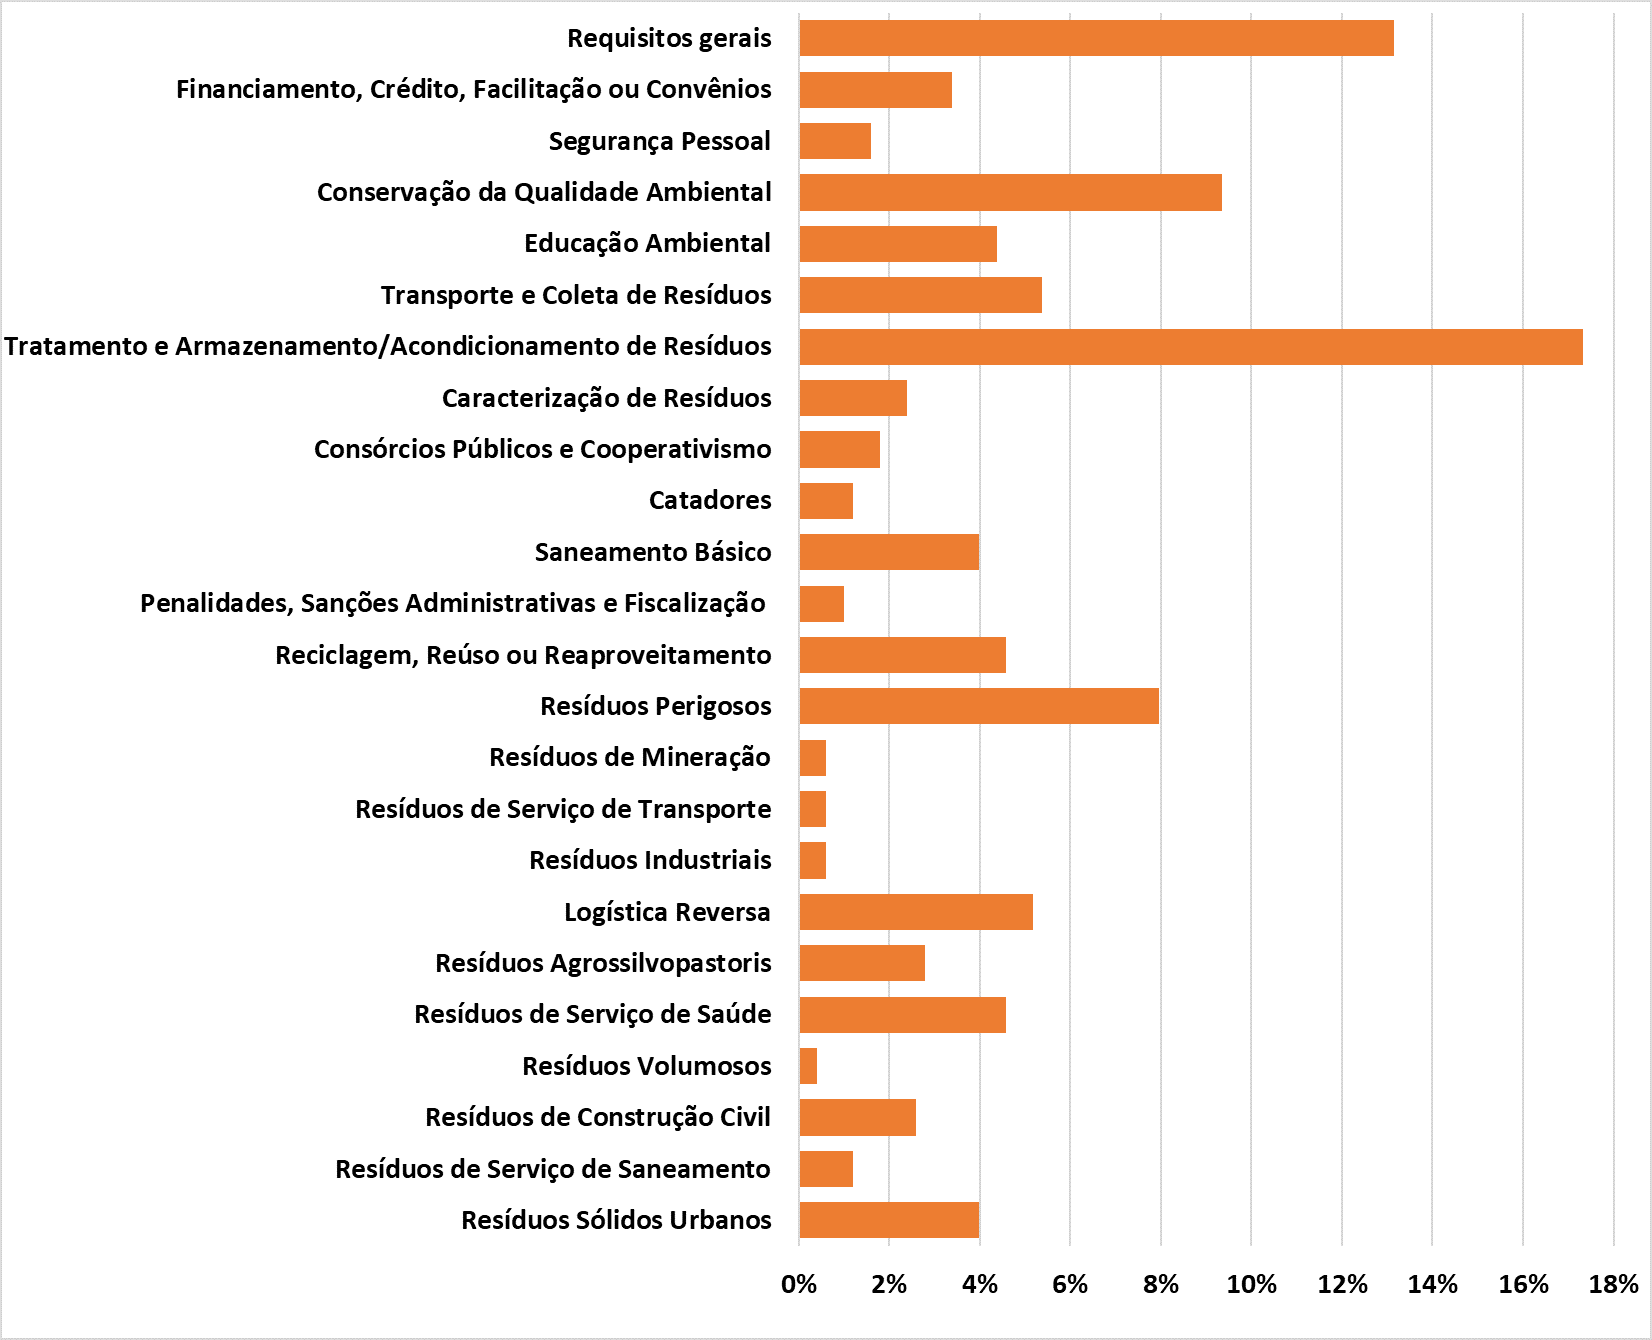
\includegraphics[width=\linewidth]{produtos/produm/distribuicaolegislacao}
		\caption{Distribuição de legislações e normas existentes por temas da gestão dos Resíduos Sólidos}
		\label{fig:distribuicaolegislacao}
	\end{figure}
	
	
	Observando a \autoref{fig:distribuicaolegislacao}, é possível verificar que a maioria das leis existentes é aplicada ao tema do tratamento e armazenamento/acondicionamento dos resíduos (17,3\% do total).
	
	Os resíduos perigosos, por sua vez, foram objeto principal de ações legisladoras, em maior parte, do governo federal. Não há, apesar do considerável número de leis de outras esferas da administração pública, nenhuma lei sobre esse tema na esfera pública municipal.
	
	Resíduos volumosos demandam grandes gastos de verbas públicas. Foi compilada apenas uma lei sobre a gestão de volumosos, municipal, que versa sobre a autorização de extrair e coletar podas de árvores volumosas ou não. Note-se que, apesar dos custos associados à gestão desse tipo de resíduos, não há nenhuma legislação específica sobre como realizar o gerenciamento de móveis, equipamentos domésticos, veículos inutilizados, entre outros.
	
	A fiscalização, juntamente com temas de sanções administrativas e penalidades, por sua vez, foi contemplada com cinco legislações em âmbito nacional e estadual e municipal, sendo apenas uma prescrita por Monteiro.
	
	Duas das legislações sobre fiscalização, uma federal e outra estadual, respectivamente, o Decreto federal Decreto 6.514/2008 e a resolução da secretaria de meio ambiente do estado de São Paulo 114/2010, versam sobre o gerenciamento de resíduos sólidos de um modo geral, com claras exigências em relação à conservação da qualidade ambiental. O único dispositivo legal municipal sobre a fiscalização, o Decreto municipal 753/1998, versa especificamente sobre a limpeza de ambientes públicos. Não há, na esfera da administração pública municipal, dispositivos legais específicos para a fiscalização de transporte, coleta, destinação final, gerenciamento de resíduos perigosos, educação ambiental, entre outros temas relevantes à gestão dos resíduos sólidos. 
	
	O tema referente à participação de catadores também foi contemplado com poucas legislações, sendo uma federal, duas estaduais e três, municipais, as quais equivalem a 1,2\% do total de leis e normas. Dentre as legislações municipais e estaduais, não há nenhuma que especifique a forma com que deve ocorrer a inclusão social e participação de catadores, o que poderia servir para detalhar assuntos abordados de forma geral pelo Programa Pró-Catador, do Decreto federal 7405/2010.
	
	A maior parte das leis e normas sobre gerenciamento de RSU foram elaboradas em nível estadual e municipal.  Diferentemente do que ocorre com os RSU, os resíduos de serviço de saneamento são quase totalmente regrados por meio de instrumentos legais e normativos em nível de federação. Os resíduos de serviços de saúde, agrossilvopastoris possuem instrumentos regulamentadores de todas as esferas de governo.
	
	Os resíduos da construção civil possuem maioria de legislações municipais. Ressalta-se a lei municipal 865/91, que versa sobre a doação de materiais de construção a famílias de baixa renda. Essa lei, caso seja implementada, poderá, ao mesmo tempo, diminuir os custos de disposição dos materiais descartados, ainda em condições de uso, e promover ganhos sociais.
	
	Os resíduos de logística reversa (pilhas e baterias, pneus, óleos lubrificantes e suas embalagens, lâmpadas fluorescentes e produtos eletroeletrônicos e seus componentes) não foram contemplados por nenhuma legislação municipal. A maior parte dos regramentos para a logística reversa foi feita pelo governo federal. Nesse contexto, percebe-se que não há detalhamentos em nível local sobre como o sistema logístico deverá ocorrer. Resíduos industriais não foram contemplados por nenhuma legislação municipal ou estadual, existindo somente em âmbito federal.
	
	De acordo com a administração municipal, serviços de transporte, tais como o transporte escolar, são indispensáveis à dinâmica econômica e cultural de Monteiro Lobato. No entanto, os resíduos gerados nesse setor, ainda não possuem regramentos específicos de gerenciamento, elaborados por ações legisladoras em nível regional ou local.
	
	Resíduos gerados por mineração não possuem leis estaduais. Além das exigências legais em nível federal, o município possui, em nível local, exigências sobre a prática de mineração e seus rejeitos gerados.
	
	